  \documentclass[12pt]{article}

  \usepackage[fleqn]{amsmath}
  \usepackage{color}
  \usepackage{listings}
  \usepackage[margin=1in]{geometry}
  \usepackage{indentfirst}
  \usepackage{graphicx}
  \usepackage{float}

  \begin{document}

  \begin{center}
  \vspace*{\fill}
  {\Large\bf University of Waterloo}\\
  \vspace{3mm}
  {\large\bf SE464 Fall 2017}\\
  \vspace{3mm}
  {\Large\bf Project Architecture and Design}\\
  \vspace{5mm}
  {\Large Project Name: WatNotes}\\
  \vspace{5mm}
  Michael Socha, Mitchell Kember, Do Gyun Kim, Myungheon Chun\\
  \vspace{3mm}
  msocha@edu.uwaterloo.ca, mkember@edu.uwaterloo.ca, dg3kim@edu.uwaterloo.ca, m5chun@edu.uwaterloo.ca\\
  \vspace*{\fill}
  \end{center}

  \newpage

  \section{Project Architecture}
  \subsection{Overview}
    WatNotes is a platform designed to allow students at the University of Waterloo to effectively upload, share
    and collaboratively edit notes. WatNotes has a mobile client used primarily for uploading notes, searching for
    other relevant notes, and other activities that tend to have short session times.
    A website is also supported for activities that require greater user commitment and focus, such as studying and
    collaboratively editing notes. \\

    Once the supported platforms for WatNotes were finalized, development was divided into three separate teams, namely
    backend, mobile, and web. The backend team is run by Mitchell Kember, and is responsible for developing WatNotes' API
    endpoints, infrastructure and data storage. The mobile team is run by Michael Socha, and is responsible for developing
    WatNotes' Android application. The web team is run jointly by Myungheon Chun and Do Gyun Kim, and is responsible for
    developing and deploying the Watnotes website. \\

    In this section, WatNotes' architecture is analyzed in a way that treats the backend, mobile client, and website of the system
    somewhat as black boxes (low level of detail). The subsequent sections expand upon each of these platforms in greater detail. A high-level component diagram where each platform is described as a separate component is described below. \\

    From a high-level overview where each of WatNotes' platforms are treated as separate components, the main architectural styles applied are
    a client-server architecture and a blackboard-based shared memory architecture. A client-server architecture is built with Watnotes' mobile
    applications and website as the clients, which are communicating with WatNotes' server through a REST API. A blackboard-based shared memory
    architecture is achieved through the system-wide data store in the backend, to which clients can upload and retrieve data, maintaining a
    global system state. \\

    \begin{figure}[H]
      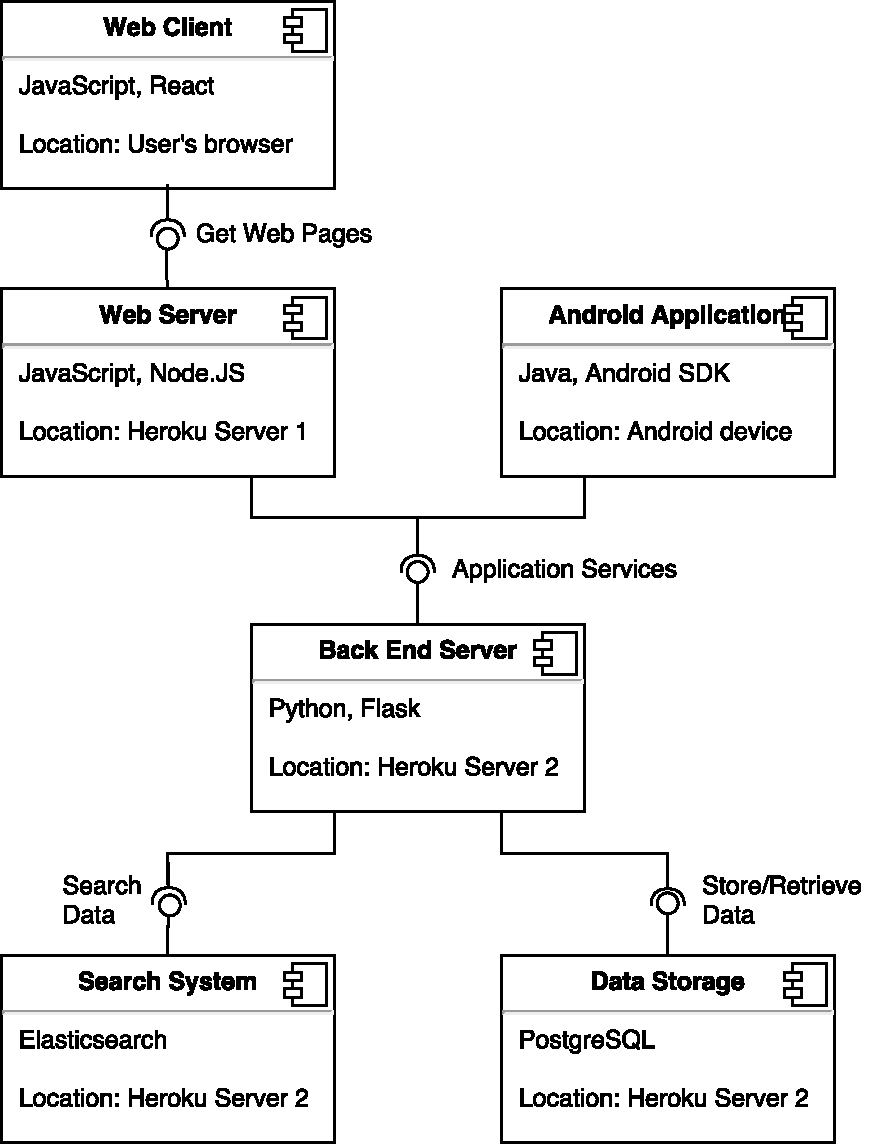
\includegraphics[width=\textwidth]{assets/overview.pdf}
      \caption{Component diagram presenting an overview of the architecture of WatNotes}
    \end{figure}

  \subsection{Backend}
    The backend of WatNotes comprises the core application logic and persistent
    data storage. Through the Backend Server, it provides the ``Application
    Services'' interface to the rest of WatNotes, namely the web application
    and the Android application. There are two main subsystems that sit
    underneath the Backend Server in the layered architecture: the Data Storage
    module and the Search System. For production, these three subsystems are
    deployed together on a Heroku dyno. All these components are shown in the
    component diagram below.

    \begin{figure}[H]
      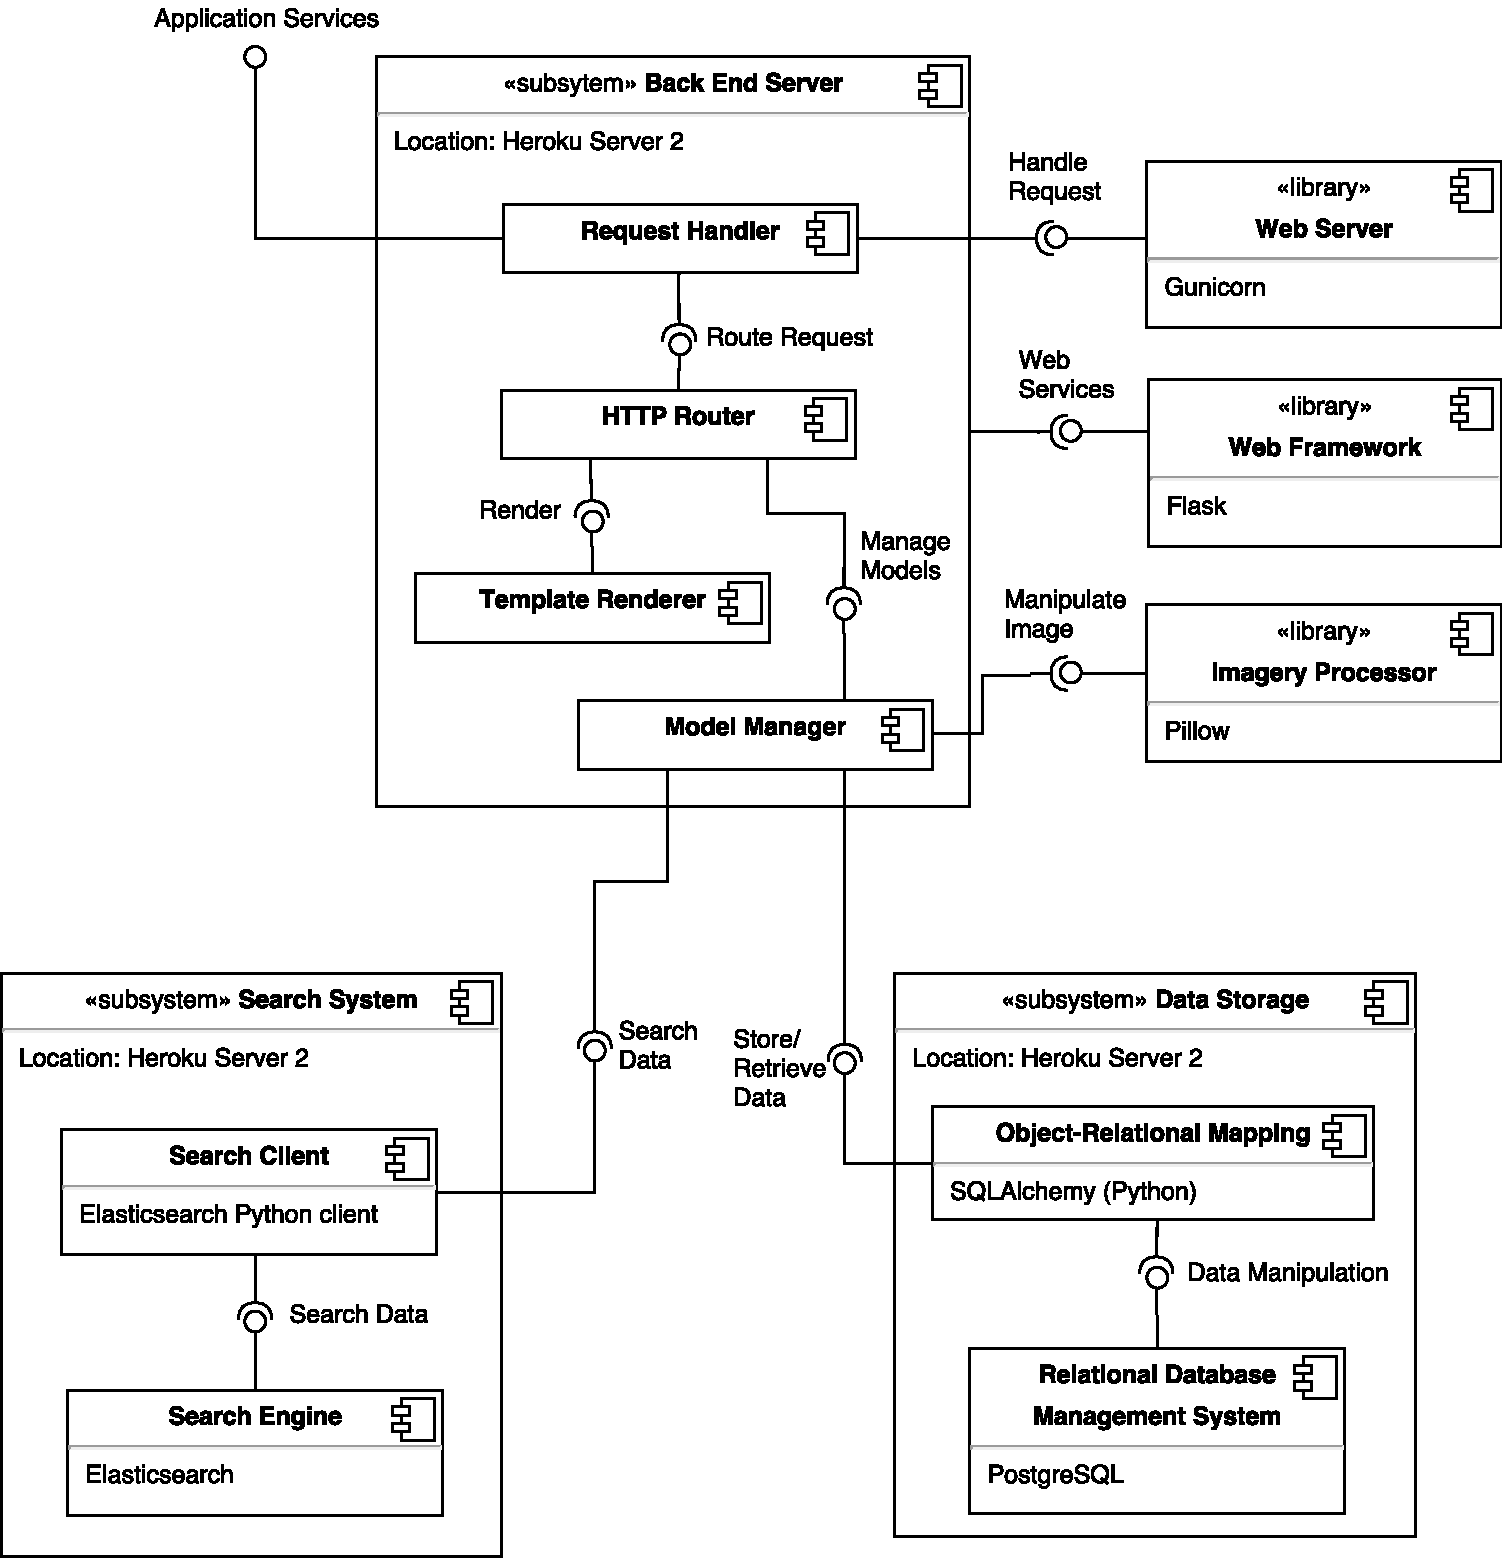
\includegraphics[width=\textwidth]{assets/backend-component.pdf}
      \caption{Component diagram showing the backend of WatNotes}
    \end{figure}

    The Backend Server is a Python application that uses the Flask web
    framework. It handles requests from clients, dispatches them according to
    URL routing rules defined in the HTTP Router component, and then accesses
    the database to produce results. In production, the Backend Server uses the
    Gunicorn HTTP server. This serves the nonfunctional property of efficiency,
    as Flask's built-in HTTP server is inefficient and only suitable for
    development. The Backend Server also uses the Pillow library for image
    processing. This is also useful for efficiency, since it allows the server
    to resize large images to more suitable sizes, making load times faster.\\

    The Data Storage subsystem consists of two parts: SQLAlchemy, a Python
    Objection-Relational Mapping (ORM) library; and PostgreSQL, a popular open
    source Relational Database Management System (RDBMS). The data that WatNotes
    stores is highly relational, so it made most sense to use an RDBMS.
    Furthermore, PostgreSQL provides the nonfunctional property of dependability
    via support for ACID-compliant transactions (atomic, consistent, isolated,
    durable). This means we can depend on the WatNotes backend to never get into
    an inconsistent state, nor to corrupt data as a result of a system outage.\\

    Instead of specifying SQL tables and queries directly, the Backend Server
    creates and manipulates Python objects (called ``Models''), and relies on
    SQLAlchemy to map these to the SQL domain. This serves the nonfunctional
    property of evolvability, since it makes it very easy to make changes at the
    data representation level with migrations and changes to the models to store
    or calculate new data.\\

    The Search System provides an efficient means of searching globally across
    all notes for specific keywords or fragments of text. It comprises a Python
    client, used by the Backend Server via procedure calls, and the Search
    Engine. The Search Engine is an instance of Elasticsearch running on a
    different port on the same machine. The redundant storage of data in both
    PostgreSQL and Elasticsearch is a small price to pay for the incredible
    speed of Elasticsearch. This also helps provides the functional property of
    discoverability, since search is a primary way to discover notes.

  \subsection{Android Application}
    The Android application is written primarily in Java, which is the most commonly used
    language in Android development. Alternatives such as Kotlin seemed somewhat immature, and
    Java meets the requirements of being object-oriented and being well-known by members of
    the group. \\

    UI layouts are primarily built using XML files, which generate layout resources
    that can be inflated at runtime. Placing the majority of UI logic in XML files helps
    separate program logic from UI construction, and XML is also known for being fairly easy to read.
    To avoid excessive duplication in UI construction, common styles, colors and dimens are
    stored in their respective resource files (styles.xml, colors.xml, dimens.xml). \\

    Since the backend communicates through a JSON-based REST API, two key components of the
    Android application are an HTTP client and a JSON parser. For the HTTP client, Square's
    OkHttp is used, and a thin wrapper is formed around its instances in the ApiRequest class.
    This library is loaded as an external dependency in the application's gradle file.
    For JSON parsing functionality, the built-in org.json package is used. \\

    The class-level organization of the Android application is described in more detail in the Design section,
    so a high-level overview is provided below. In short, each Activity (the fundamental building block of Android apps)
    has an associated UiFragment and ServiceFragment. UiFragments are responsible for initializing and managing the UI
    for an activity, while ServiceFragments are responsible for handling all of an activity's networking calls. A common
    execution sequence is that the UiFragment makes a request to a ServiceFragment, which in turn makes a call to
    the UiFragment to update its UI based on the returned information (e.g. to populate a feed). \\

    A high-level overview of the functional components of the Android application is shown below: \\
    \begin{figure}[H]
      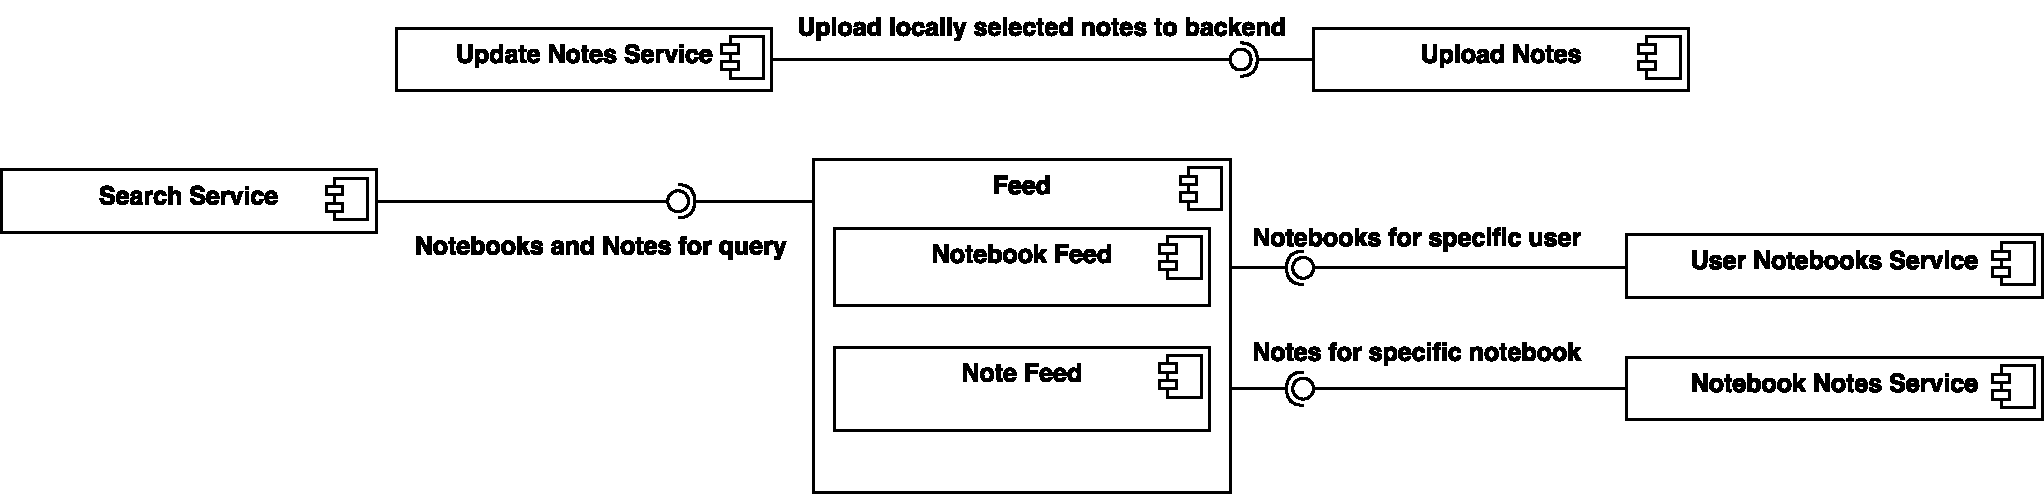
\includegraphics[width=\textwidth]{assets/android-arch.pdf}
      \caption{Architecture of WatNotes Android application}
    \end{figure}

  \subsection{Website}

  The front-end architecture consists of mainly three components: Login, Feed and Note. As the name suggested, the login component is responsible for authenticating the user via acquiring JWT from the web server. Feed Component handles all the main actions which users can perform in our application. The actions include discovering the user's customized notes and searching through specific notes via tagging. Finally, note component is where users can view and edit the published notes and collaborate with other users. \\

  \begin{figure}[H]
    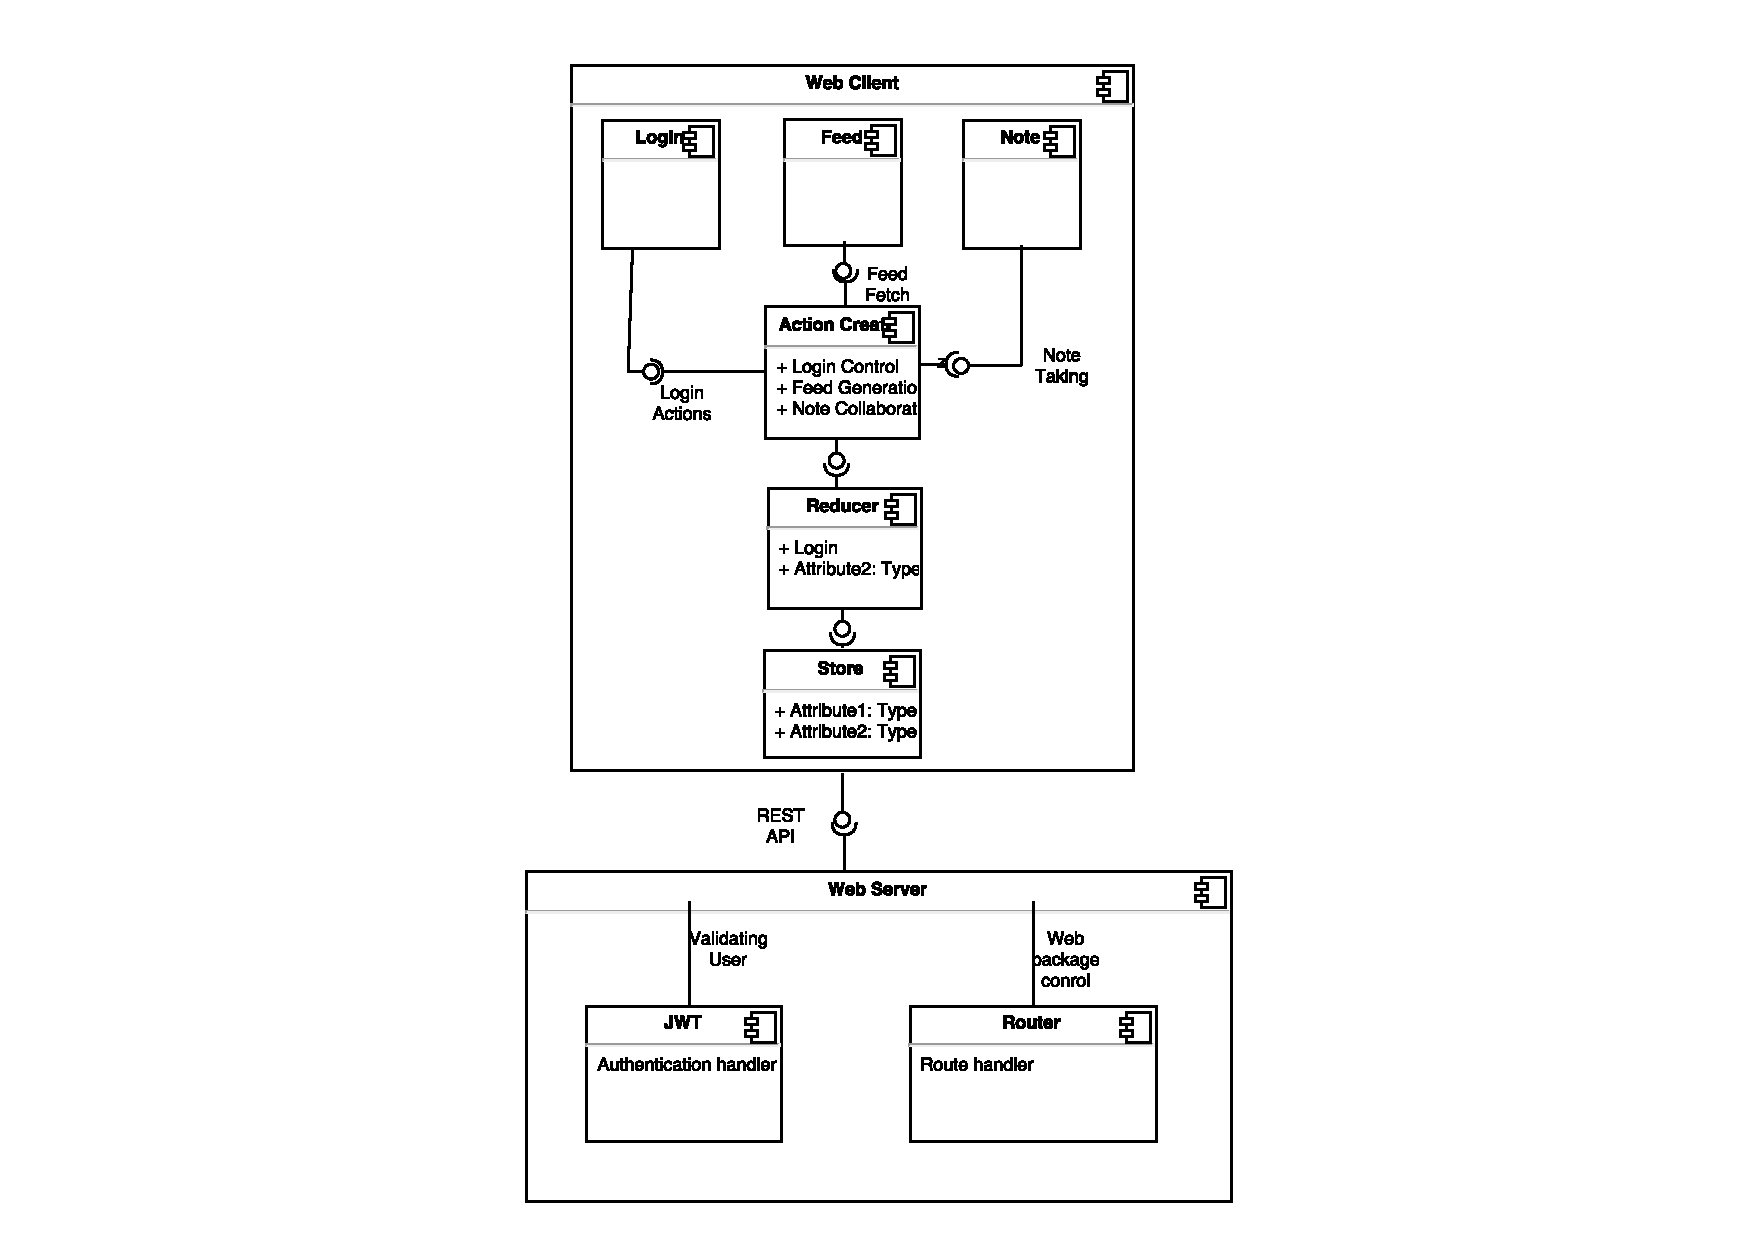
\includegraphics[width=\textwidth]{assets/frontend_architecture.pdf}
    \caption{Architecture of WatNotes Front-end}
  \end{figure}

  Our architecture must be open to adapt rapid product requirement changes. We thought react and redux architecture style would be an ideal choice to achieve the goal. Redux architecture is similar to blackboard shared memory architecture. Essentially, we have many components that are listening to one centralized data source called, store. Store can often be referred as a state of an application that is an immutable object which cannot be manipulated by external functions. In redux model, a new store is created by actions. Actions are what components dispatch when users perform certain inputs each component is listening to, then reducer handles the action through merging the result of the action into the old state to produce a new state. Since it is based on components or a hierarchy of components, we can easily remove or add new components to fulfill our needs. Another benefit is reusability. Not only we can add or remove those components, we can reuse them elsewhere. For instance, if we would like to reuse the display of notes in feed page in note page, we can do so through simple call to the component in note page. Hence, the flexibility and reusability in our architecture would help us to build an evolvable architecture. \\

  The application is built upon the trust from users on the confidentiality, integrity and availability of their data. To have it fault tolerant, the system should be close to bug free. One thing which react gives us is transparency. We can clearly see how the application transition to one state to another through serious of actions and reducing. Hence, it is resistible to implementation failures, given there is little to none design flaws. One of key functional property is discovering internet scale published notes and collaborate with multiple users in real-time. Therefore, the application must be efficient and responsive. Unlike many other heavyweight frameworks like AngularJS or BackboneJS, react is lightweight in an absolute measure. This frees us from heavy abstraction from the framework which can be sometimes cumbersome. For instance, to do simple synchronization or data sharing between components in AngularJS it must be done through broadcast feature. The problem arises when there are too many communications between components and due to limited functionalities, it can get very hairy. However, since we are not relying on heavy abstraction and building them from scratch, we can be  creative with our design and implementation to optimize performance of the application. \\


  \newpage

  \section{Project Design}
  \subsection{Backend}
    As mentioned in the architecture section, the Backend Server of WatNotes is
    a Flask application, written in Python. The use of Flask largely dictates
    the design of the application, since for most of its use cases their is a
    prescribed method and style for achieving it.

    The design can be separated into three main parts: the HTTP router, the CRUD
    helpers, and the Models. The router defines a REST API by mapping different
    URLs and HTTP verbs to either queries of manipulations of the database. It
    performs these queries and manipulations view the CRUD (create, read,
    update, delete) helpers, which are located in a separate module and
    implement generic routines for manipulating all the Models. These routines
    include getting a specific record, updating attributes of an existing
    record, creating a new record, and listing all records of a given type in a
    paginated fashion. Both the router module and the CRUD module follow a
    functional style of programming, without the use of classes, and so there is
    no class diagram for them. The Models, however, are organized in a class
    hierarchy shown in the figure below:

    \begin{figure}[H]
      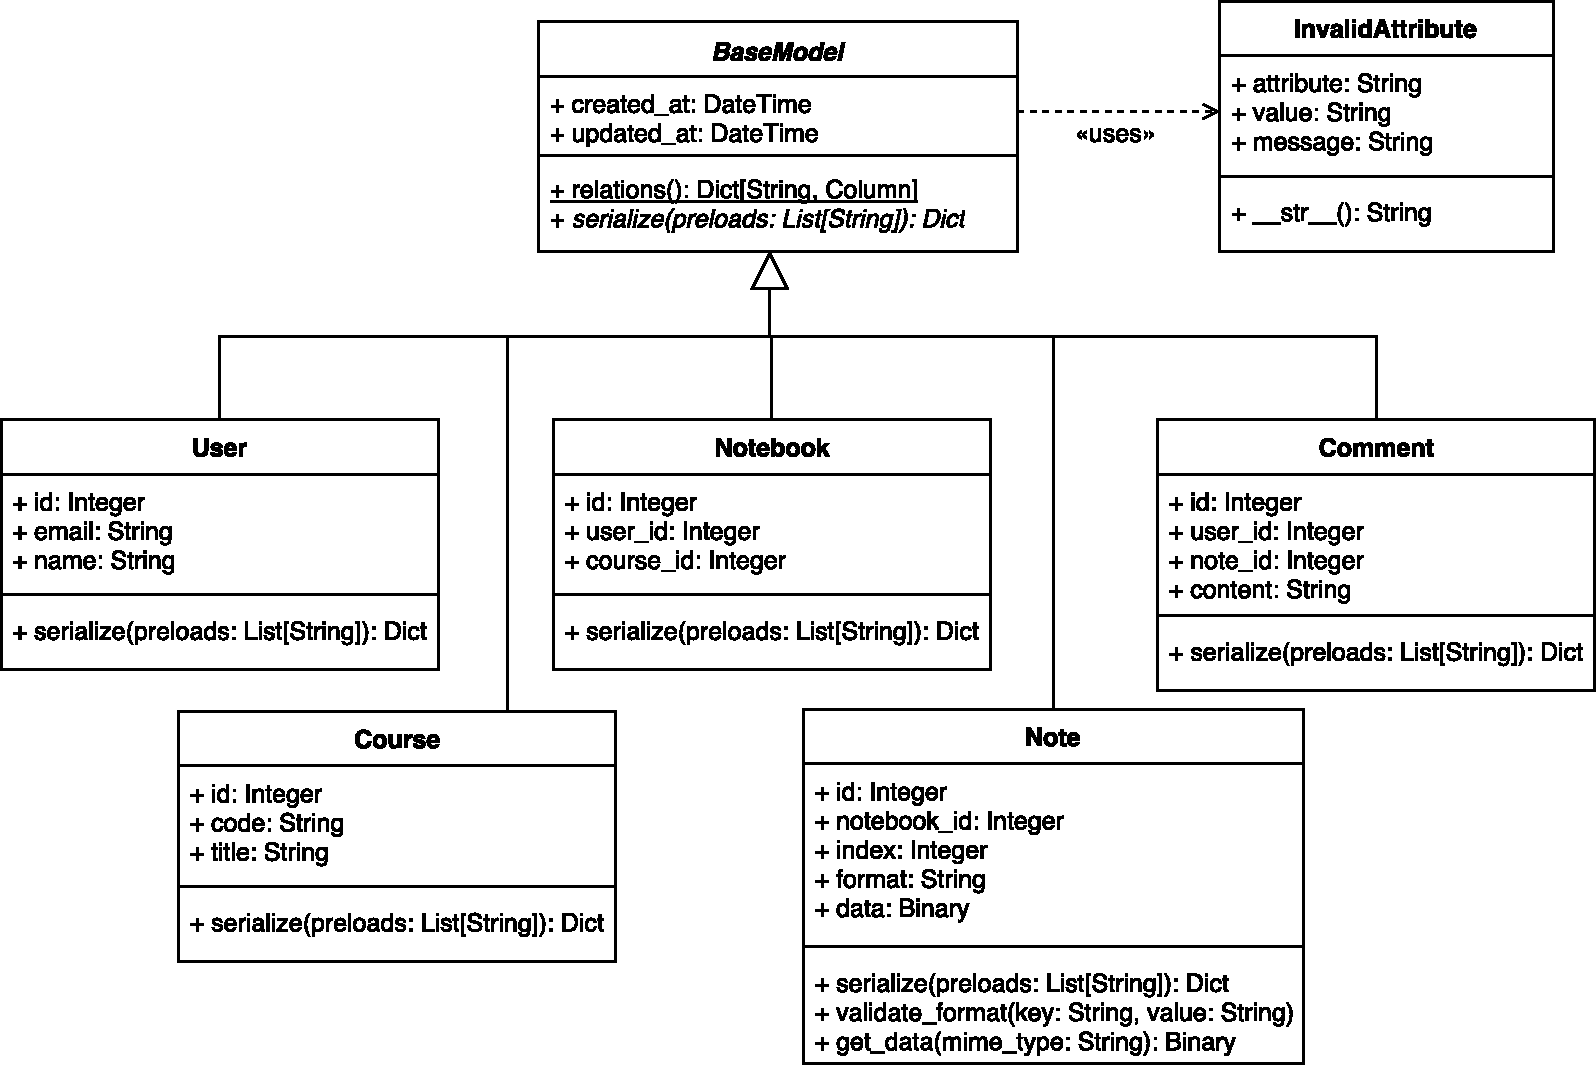
\includegraphics[width=\textwidth]{assets/backend-class.pdf}
      \caption{Class diagram diagram of the Python backend server of WatNotes}
    \end{figure}

    All Models inherit from BaseModel, which defines common attributes and
    methods. For example, every Model in the database has columns called
    ``created\_at'' and ``updated\_at,'' which are automatically set on creation
    and upon updating. In addition, the Models use the Observer design pattern
    to execute additional code when different events SQLAlchemy's ORM lifecycle
    occur. For example, before inserts and updates are committed, the Note class
    checks the data it is about to store, and if it is an image, it first
    processes the image to resize it and convert it to a desirable format.

    In addition to Note, there are four other Models: User, Course, Notebook,
    and Comment. Their relationships are as follows: each User can have many
    Notebooks, each corresponding to a particular course; within a Notebook
    there exists many Notes; and a particular Note may have many Comments on it,
    each associated with a User. Each implements the ``serialize'' method to
    convert their data to JSON form, so that the HTTP router can respond to the
    client with JSON data. In addition, these functions support
    \emph{preloading} other records, so for example a request to get a User may
    preload all the users Notebooks in a single query.

  \subsection{Android Application}
    This section serves to provide a general overview of the Android application's class-level design. All of the described components run on the Android
    device on which the application is operating (no distributed logic). \\

    One major design decision of the app concerns how the application handles Android's activity lifecycle. In short, activities are the basic building blocks of
    an Android app, providing a user with a UI, resource management and handling for certain OS events. Much of this logic is common to all activities, and
    hence is abstracted into a common BaseActivity class. BaseActivity is an abstract class that follows a template design pattern, with functionality
    such as getting the UI layout container (getLayoutId) and initializing the UI once it is loaded (setupUi) implemented by concrete subclasses. DrawerActivity
    is an abstract subclass that extends from BaseActivity, and implements a side navigation drawer - most activity classes in WatNotes inherit from DrawerActivity. \\

    Each activity must implement the createUiFragment and createServiceFragment methods. UiFragments implement an activity's UI (e.g. loading and
    initializing layout resources), while ServiceFragments are responsible for handling an activity's networking by providing an interface
    to service instances (adapter design patter). The BaseActivity attaches both of these fragments to the activity, where they can have independent sub-lifecycles
    within the activity. UiFragment and ServiceFragment are both abstract base classes, with concrete UiFragment and ServiceFragment instances associated with each
    concrete class. \\

    \begin{figure}[H]
      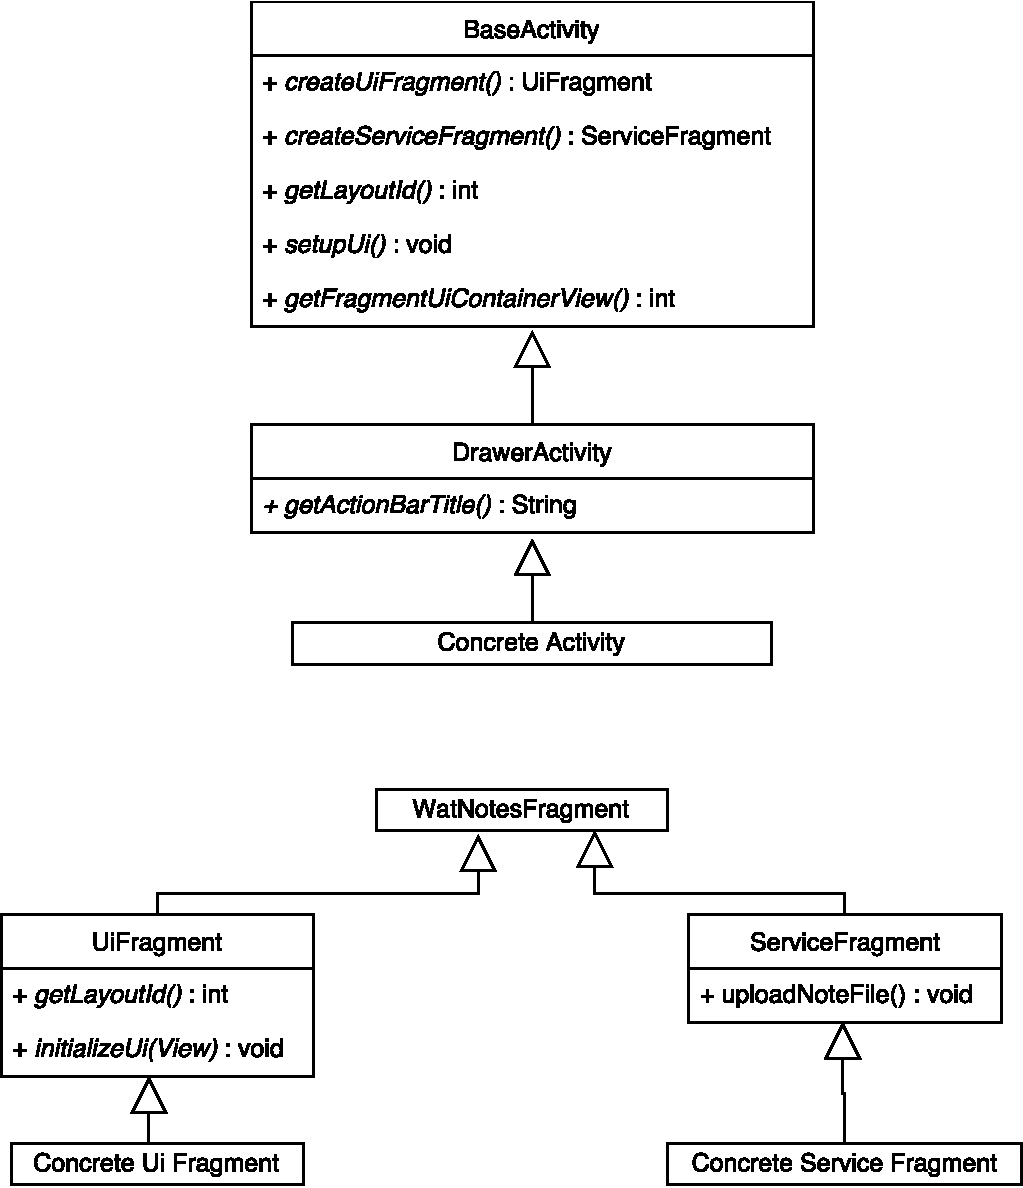
\includegraphics[width=\textwidth]{assets/android-activity-class.pdf}
      \caption{Class diagram diagram of the Android application's activity and fragment design}
    \end{figure}

    Another major design decision concerns how the app's networking layer is organized. An abstract base class called ApiRequest defined from which the abstract
    SingleApiService and MultiApiService classes extend. SingleApiService classes are services for which there are never expected to be more than one active request. Thus, whenever
    a service is started through a call to startRequest(), any pre-existing service is canceled. On the other hand, MultiApiServices may have multiple requests active,
    and a request is only canceled in calls to startRequest() if it shares the requestId of the new request. Concrete ApiRequest classes extend from either
    SingleApiService or MultiApiService classes, following a template design pattern. \\

    \begin{figure}[H]
      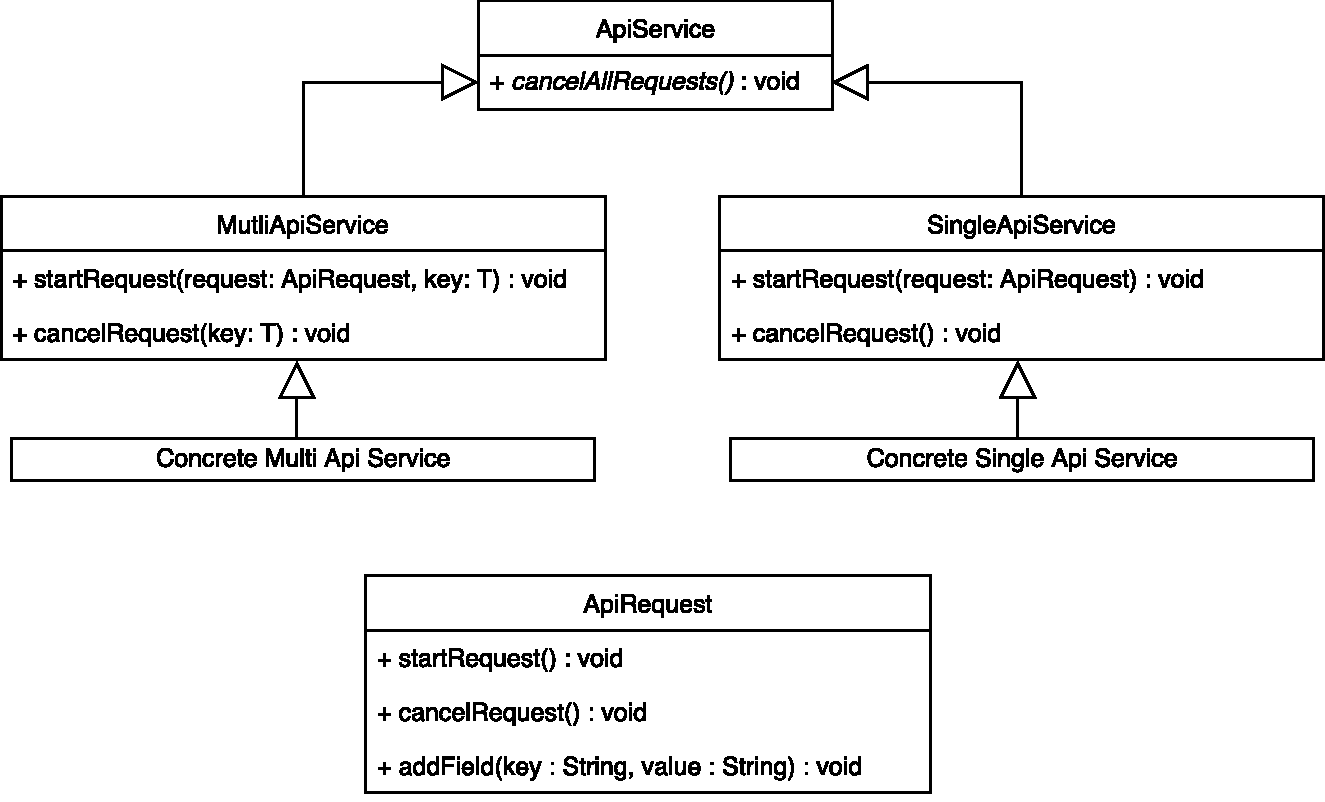
\includegraphics[width=\textwidth]{assets/android-network-class.pdf}
      \caption{Class diagram diagram of the Android application's networking and service design}
    \end{figure}

    As shown by the examples above, the design of the Android application relies heavily on the template design pattern to abstract away common functionality. This can help
    accommodate future requirements by speeding up and simplifying the development of new activities, fragments and services. Moreover, where applicable, the Android application
    favours composition over inheritance. For instance, some feed views (e.g. the notebook feed view) support a custom callback for when a notebook is selected, allowing the same
    feed to be used for multiple purposes. Favouring composition over inheritance tends to increase the flexibility and evolvability of the application, allowing it to effectively
    accommodate a variety of future features. \\

    Organizing the application as single-purpose classes helps increase cohesiveness. Coupling is decreased through the use of well-defined, high-level interfaces (often enforced
    through the template design pattern).

  \subsection{Website}
  The front-end of WatNotes is a react-redux application that runs on a node server and uses webpack for dependency management. The source code for the project is under the src directory. In src, the main index.js file can be found which initializes the react router and redux store. Other important subdirectories in the src directory include store, containers, and components. Any new dependencies required in the project are handled using npm and should be added to the webpack build as required (look in the webpack directory).\\

  The react router implements the logic for deciding which components to render based on the url. When the browser goes to a specific url, a container is chosen to render. The react router is an example of the strategy design pattern. Containers define the data that will be passed down to components to render. They define the data to be passed down by referencing the redux store and are responsible for actions such as fetching data from an api and bootstraping the components with the fetched data. This is an example of one way directional data flow where components only receive data and cannot modify the data received. This pattern decreases complexity since the developer only has to manage 1 data state (the redux store) and can think of components as only having the responsibility of rendering the ui (single responsibility principle). A component is a class that represents what you see visually only. Components are designed to be reusable and has no dependencies other than the properites passed into the class constructor. This minimizes coupling as ui components have no dependencies and it also maximizes flexibility which helps accommodate for future requirement changes. If a new ui component or an existing requirement for a ui component is changed, minimal changes are needed since the UI would be broken up into small components.\\

  The use of react and redux separates the the ui logic from the data state logic. Redux containers can fetch data using the backend api and pass it down to the components. As more features are added, more properties will have to be added to the state along with more containers to decide how to pass down those new properties down to components. Since there is a single store, adding more data to the store will not affect other parts of the application.

  \begin{figure}[H]
    \centering
    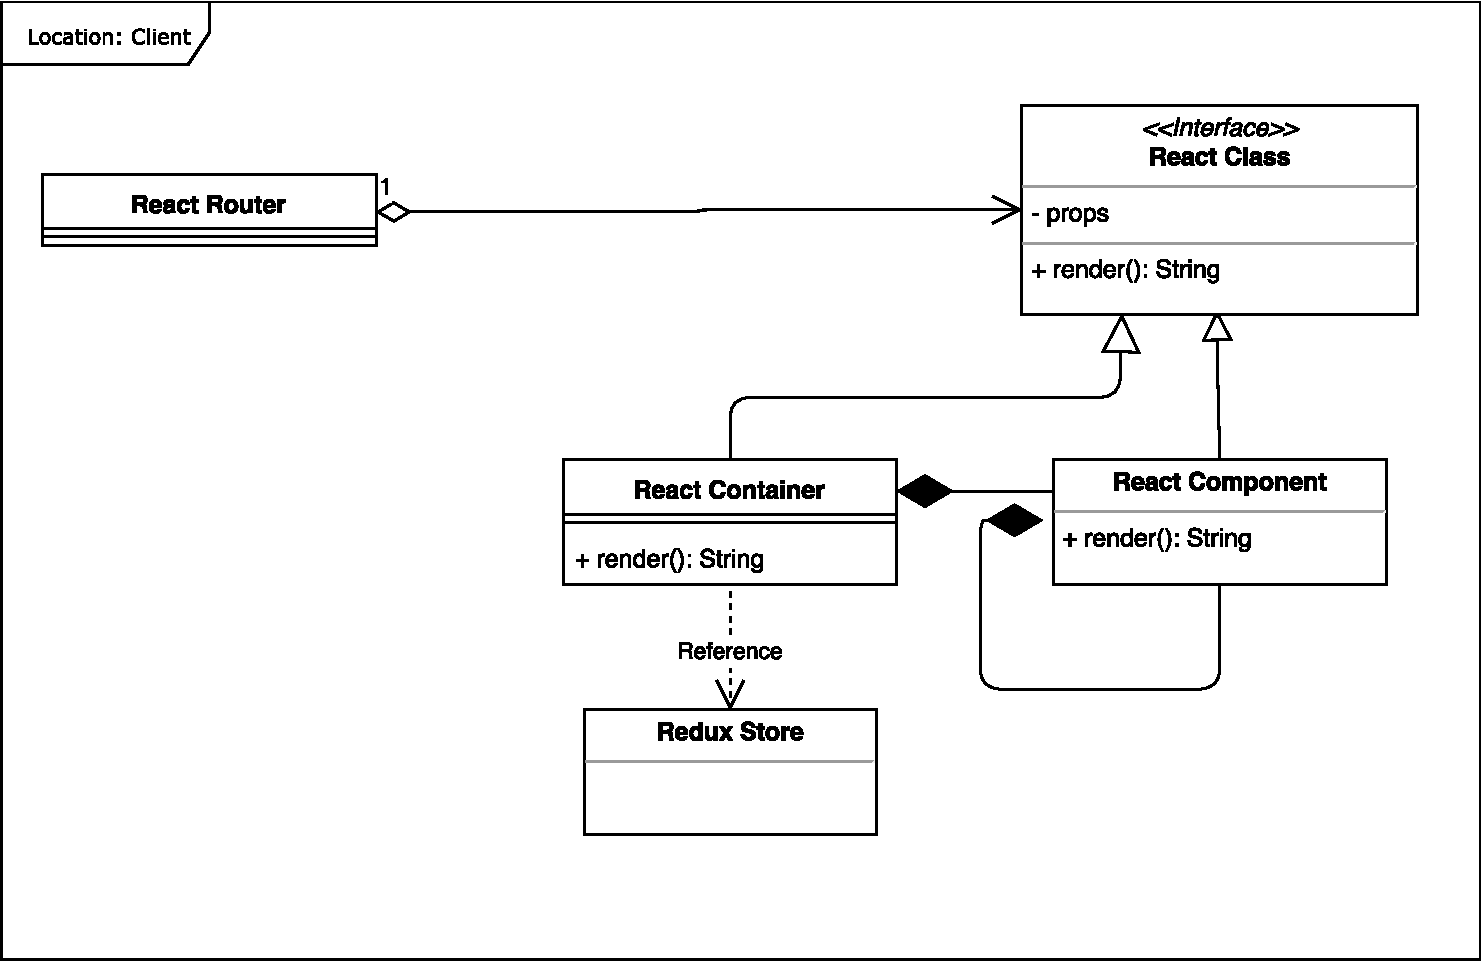
\includegraphics[width=\textwidth]{assets/frontend_design.pdf}
    \caption{Class diagram of the website design of WatNotes}
  \end{figure}

  \subsection{Sequence Diagrams}
    Below are two sequence diagrams based on the two use cases defined in the application's prescriptive architecture.

    \subsubsection{Student uploads notes}

    \subsubsection{Student receives feedback on uploaded notes}

  \newpage

  \section{Participation journal}
    \subsection{Mobile}
      Michael Socha was responsible for developing the mobile (Android) application for the project. The mobile architecture, design and implementation-level artifacts
      have been built by him.
    \subsection{Backend}
      Mitchell Kember was responsible for the backend server. He built the
      Python app using Flask, and configured PostgreSQL and Elasticsearch to
      work with the server. He also deployed the backend to Heroku, so that the
      web client and mobile application could run against the same backend.
    \subsection{Web}
      Justin Kim was responsible working on feed, search and login portion of the front-end. He was also layed out the general structure
      of the front-end architecture. 

      
      Myungheon Chun
    
\end{document}
